\documentclass[12pt,a4paper,titlepage]{article}
\usepackage[a4paper,left=25mm,right=15mm,top=20mm,bottom=20mm]{geometry}
\usepackage[utf8]{inputenc}
\usepackage[L7x]{fontenc}
\usepackage[lithuanian]{babel}
\usepackage{amsmath}
\usepackage{amsfonts}
\usepackage{amssymb}
\usepackage{setspace}
\usepackage{mathptmx}
\usepackage{graphicx}
\usepackage{float}
\onehalfspacing
\usepackage[backend=biber, style=apa, url=false, sorting=nyt]{biblatex}
\addbibresource{bibliography.bib}
\title{Pajamų nelygybė: formavimasis ir mažinimo metodai}
\author{Tomas Dzedulionis}
\date{2019m. Birželio 18d.}
\begin{document}
\maketitle
\newpage
\setcounter{tocdepth}{3}
\setcounter{secnumdepth}{3}
\tableofcontents
\newpage
\section{Įvadas}
Pajamų nelygybė - viena opiausių ir vis dar sparčiai besivystanti problema, kurios mastas kasmet didėja. 2007-2008m. finansinė krizė kirto skaudžiai, iki tol sparčiai augusi Europos ir pasaulio ekonomika smuko ir dar nepasiekė prieš krizinio lygio. Remiantis World Inequality Lab pateikta 2018m. pasauline pajamų nelygybės ataskaita(\cite{alvaredo2018world}), galime matyti, jog paskutiniaisiais dešimtmečiais pajamų nelygybė augo praktiškai visose šalyse, o ypač tai pastebima rytų Europos valstybėse. 1 procentas pasaulio turtingiausiųjų valdo 45 procentus viso pasaulio turto. Pajamų nelygybė šalyse, priklausančiose OECD (Tarptautinė ekonominio bendradarbiavimo ir plėtros organizacija), siekia aukščiausią tašką per paskutinį pusę amžiaus. Nepasitenkinimas didėjančia pajamų ir socialine atskirtimi vis auga. Visuomenė stebi procesą, kurio metu vis didesnė dalis turto kaupiama turtingiausiųjų rankose, auga skurstančiųjų skaičius, o vidurinioji klasė pamažu nyksta. Augantis žmonių nepasitenkinimas virsta ne tik aiškiais veiksmais ( pvz.: geltonųjų liemenių judėjimas Prancūzijoje), tačiau taip pat sudaro sąlygas kilti populistinėms partijoms, o tolimesnis problemos nesprendimas gali turėti katastrofiškų padarinių. 

\section{Pajamų nelygybės formavimasis}
\subsection{Istorinė seka}
Klausimas kaip formuojasi ir vystosi pajamų nelygybė, ekonomikoje, kaip mokslo šakoje, yra nagrinėjamas daugiau nei visą amžių, tačiau santykis tarp pajamų nelygybės proceso formavimosi ir jo padarinių vis dar neišaiškintas. Iki maždaug 2000-ųjų metų pajamų nelygybės klausimas sprendėsi tarp dviejų pagrindinių teorijų (\cite{aghion1998growth}):
\begin{enumerate}
\item Pajamų nelygybė yra gera skatinamoji priemonė, todėl prisideda prie ekonomikos augimo. 
\item Kuznets'o (Nobelio premijos laureatas, JAV ekonomistas) teorema, kuri teigia, jog ekonomikai augant pajamų nelygybė didėja, kol yra pasiekiama tam tikras išsivystymo lygis, kuomet ji pradeda mažėti.  
\end{enumerate}
Teorijų pagrindimui buvo pradėta nagrinėti korealiacija tarp BVP (Bendrojo Vidaus Produkto) ir pajamų nelygybės, matuojamos GINI indeksu (Gyventojų pajamų pasiskirstymo statistinis rodiklis. Visiška pajamų lygybė Gini=0, visiška pajamų nelygybė Gini=100). Mokslininkai, atlikdami tyrimus (\cite{alesina1994distributive}) atrado, jog egzistuoja neigiamas sąryšis tarp ekonomikos augimo ir pajamų nelygybės, todėl galiausiai buvo apsistota ties antrąja teorija. Tačiau ji priimta tik dalinai, kadangi Kuznets'o teoremos dalis, sakanti, jog egzistuoja išsivystymo lygis, kuomet pajamų nelygybė pradeda mažėti, nėra visiškai teisinga ir iki galo įrodyta.  
Istoriškai nelygybės veiksnys pastebėtas jau Mesopotamijoje ar senovės Egipto civilizacijoje, tačiau tais laikais tai buvo panašiau ne tik į pajamų, tačiau bendro turto nelygybę. Pajamų nelygybė labiausiai atsiskleidė tik naujaisiais laikais, XVI-XVIIa Kapitalistinės sistemos pradžioje. Jau XVIIIa. klasikinės politinės ekonominės filosofijos tęsėjas, prancūzas Ž.Ž. Ruso įžvelgė besiformuojančius sistemos trūkumus ir savo filosofiniuose raštuose nagrinėjo pilietinę visuomenę. Pagal Ruso, bendruomenė iš prigimtinės būklės perėjusi į pilietinę/valstybinę formą įteisina nelygybę ir turtingųjų apsaugą, o privatinę nuosavybę paverčia pačiu didžiausiu konkurencijos objektu. Turtingieji, siekdami daugiau turto, išnaudoja vargšus ir moka šiem mažą dalį atlygio, likusį perviršį pasiimdami sau. Ruso mintys patvirtina to laikmečio Prancūzijos situacija, XVIIIa. pabaigoje nelygybė Prancūzijoje išreikšta GINI koeficientu siekė 0.59 (\cite{morrisson2000income}), o tai buvo viena iš didžiosios Prancūzijos revoliucijos priežasčių. Ruso mintys apie nelygybę ir darbininkų (proletarų) išnaudojimas industrializacijos metu įkvėpė XIXa. vokiečių filosofą, marksizmo pradininką K.Marksą. Marksizmas - ideologija, kurios pagrindiniai poliai - visuotinė lygybė ir privatinės nuosavybės panaikinimas ją išdalinant visiem (valstybei). Marksizmo praktiku tapo V.Leninas ir SSRS. Kitas radikalus atvejis, nacių partijos iškilimas Vokietijoje, kai nepasitenkinimas didele atskirtimi bei gyvenimu krizės metais sudarė sąlygas į valdžią ateiti Naciams. Tai patvirtina ir nagrinėjamas grafikas (žr.pav.1), kuriame matome staigiai kylantį GINI indekso reitingą tarpukario metu. Istorinių pavyzdžių nagrinėjimas įrodo faktą, jog pajamų nelygybės problema gali turėti kritinių padarinių.
\begin{figure}[H]
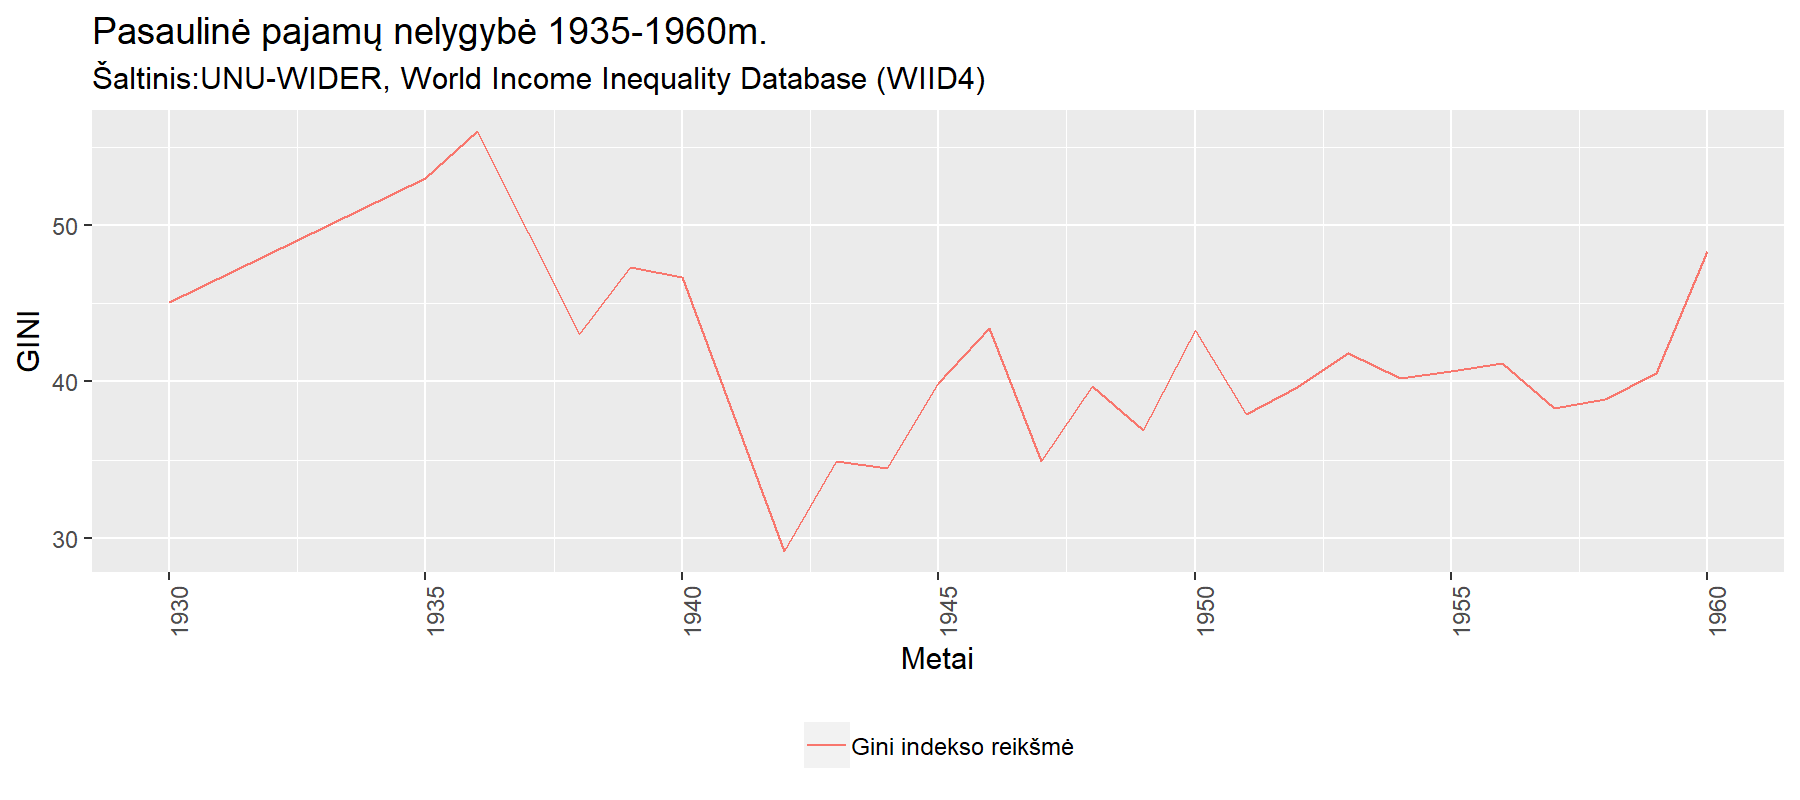
\includegraphics[scale=0.7]{historicalinequality3560.png}
\caption{Pasaulinė pajamų nelygybė 1935-1960m.}
\end{figure}
\subsection{Svarbiausi veiksniai}
\subsubsection{Neoliberalizmas ir globalizmas}
Neoliberalizmo sąvoka. Neoliberalizmas - ekonominės politikos modelis, remiamas laisvos rinkos ir valstybės dereguliacijos principais. Pagrindinė varomoji jėga - žmonių konkurencija. Ši ideologija teigia, kad valstybinio sektoriaus kišimosį į ekonomines ir socialines sferas mažinimas kartu su darbo ir finansų rinkų dereguliacija bei tarptautine prekyba ir investicijomis, išlaisvino begalinį kapitalizmo potencialą visuomenės gerovei kurti (\cite{navarro2007neoliberalism}).
Pagrindiniai neoliberalizmo principai:
\begin{enumerate}
\item Valstybė turi mažinti ekonomikos reguliavimą (mažinti mokesčius, privatizuoti valstybines įmones).
\item Darbo ir finansų rinkos turi būti dereguliuotos tam, kad atskleisti pilną laisvos rinkos potencialą.
\item Prekyba ir investicijos turi būti skatinamos naikinant trukdžius ir barjerus bei leidžiant prekėms, paslaugoms ir kapitalui laisvai judėti. 
\end{enumerate}
Visa tai prisidėjo prie globalizmo plėtros, kas, anot neoliberalizmo šalininkų, leido pasiekti naują globalaus ekonominio augimo lygį, kuris susijęs su nauju socialiniu progresu (\cite{navarro2007neoliberalism}).
Neoliberalizmo ir nelygybės santykis. Konkurencijos ir dereguliacijos varoma ideologija nelygybę iškelia kaip natūralų veiksnį - kiekvienas gavo tiek, kiek nusipelnė ir pats prisidėjo prie visuomenės gerovės. Atmetami tokie faktoriai kaip starto pozicija, kai žmogus, gimęs turtingesnėje šeimoje turi geresnes galimybes baigti mokslus, bendrauti su aukštesnes pareigas užimančiais žmonėmis ir gauti geriau apmokamą darbą. Tokį požiūrį patvirtina ir atliktas tyrimas (\cite{gilens2005inequality}), kurio metu atrastas neigamas sąryšis tarp skurstančiųjų požiūriu socialiai teisingų įstatymų priėmimo ir JAV kongreso narių balsavimo elgsenos. Vienas pirmųjų ir žymiausių neoliberalizmo praktinių įgyvendintojų buvo JAV prezidentas R.Reagan'as. Jo kadencijos metais (1981-1989) priimtų neoliberalių reformų rezultatas, remiantis pateiktu bendrų vidaus pajamų atskirties tarp 10proc. turtingiausiųjų ir 50proc. žemiausias pajamas gaunančių piliečių grafiku (žr.pav.2), atskirtis drastiškai išaugo. Tapo aišku, kad neoliberalizmo efektas - turtingieji tampa turtingesniais, vargšai - vargingesniais (\cite{martinez1997neoliberalism}). Tai iššaukė būtent neoliberalios reformos, kurias priėmė Reagan'as ir iš ko atsirado naujas terminas - \textit{reagonomics}:
\begin{enumerate}
\item Mokesčių mažinimas
\item Valstybinių išlaidų mažinimas
\item Valstybės reguliacijos mažinimas
\item Pinigų pasiūlos mažinimas siekiant mažinti infliaciją
\end{enumerate}
Neoliberalistinės idėjos ir laisvas, nevaržomas kapitalo judėjimas iššaukė ir kitą ekonominės plėtros veiksnį - globalizmą. Žiūrint iš vienos perspektyvos, globalizmas atvėrė duris globaliam verslui ir pasaulinės ekonomikos apjungimui bei ivairiausių šalių integracijai, tačiau žvelgiant iš ekonominės nelygybės pusės, globalizacija dar labiau išryškino šią problemą. Egzistuoja 5 pagrindiniai globalizmo veikimo poliai (\cite{brian2015oecd}):
\begin{enumerate}
\item Technologijos ir informacija
\item Tarptautinė prekyba 
\item Gamybos skaidymas pagal regionus
\item Laisva žmonių migracija
\end{enumerate}
Laisvas šių veiksnių veikimas atveria galimybes tarptautiniam bendradarbiavimui, tačiau vis sparčiau tobulėjančios technologijos ir augantis informacijos kiekis naikina daugelio žmonių darbo vietas tuo pačiu augant didesnių technologinių įgūdžių reikalaujančių darbų užmokesčiui. Tarptautinės prekybos poveikis pajamų nelygybei priklauso nuo prekiaujančių šalių išsivystymo lygio, tačiau galime teigti, kad pajamų pasiskirstymui efekta ji tikrai turi, nes keičia prekių pasiūlą ir paklausą, o kartu ir gamybos poreikį prekiaujančioje šalyje, bei darbo jėgos užimtumą (\cite{misiukonyte2013globalizacijos}).

\begin{figure}[H]
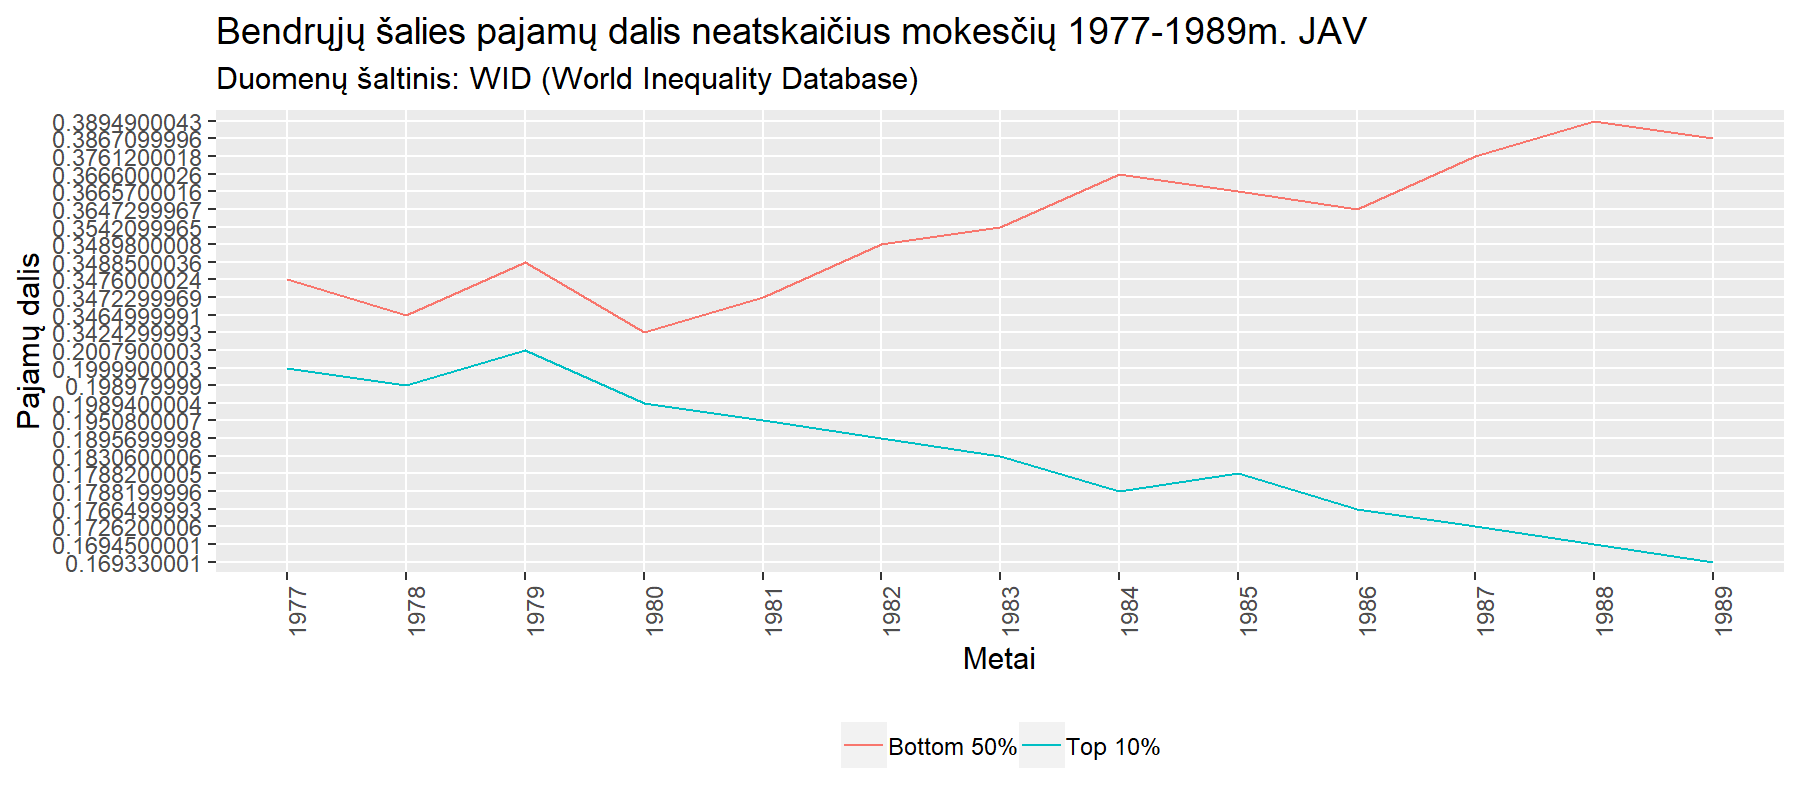
\includegraphics[scale=0.7]{top10bot507789.png}
\caption{Bendrųjų šalies pajamų dalis neatskaičius mokesčių 1977-1989m. JAV}
\end{figure}

\subsubsection{Mokestiniai veiksniai}
Vis labiau ryškėjanti ekonominės nelygybės problema verčia vyriausybės galvoti apie vis didesnį valstybės vaidmenį šioje kovoje. Tačiau daugelį metų iki tol vyravęs įsitikinimas, jog mažesni mokesčiai skatina ekonomikos augimą, didina produktyvumą ir tuo pačiu prisideda prie bendrojo gėrio iš tiesų yra klaidingas ir didina pajamų atskirtį. Progresyvių mokesčių klausimas - neišsenkanti tema. 2017metais JAV prezidentas D.Trumpas sumažino daugelį mokesčių tarifų, ypač tai pasijautė verslo korporacijoms skirtų mokesčių sumažinimui nuo 35 iki 21proc. Taip pat sumažintas ribinį individualių pajamų mokestį nuo 39.6 iki 37proc. Nors JAV ir egzistuoja progresyvi mokesčių sistema, tačiau toks mokestinės naštos mažinimas neleidžia sistemai efektyviai kovoti su pajamų nelygybės problema. Socialiai neatsakingų sprendimų priėmimą atspindi ir (M.Gilens) tyrimas, kurio metu nustatyta, jog egzistuoja neigiamas sąryšis tarp ekonomiškai skurdesnių socialinių grupių poreikių ir JAV kongreso narių priimamų sprendimų, kurių priėmimui didesnę įtaką daro turtingesniųjų pozicijos.
Remiantis pateiktu grafiku (žr.pav.3), galima daryti išvadą, jog mažėjant mokestinei naštai didesnes pajamas gaunantiems asmenims - pajamų nelygybė didėja, todėl progresyvi mokesčių sistema su aukštesniais ribiniais mokestiniais tarifais didesnes pajamas gaunantiems žmonėms galėtų padėti spręsti šią problemą. 
\begin{figure}[H]
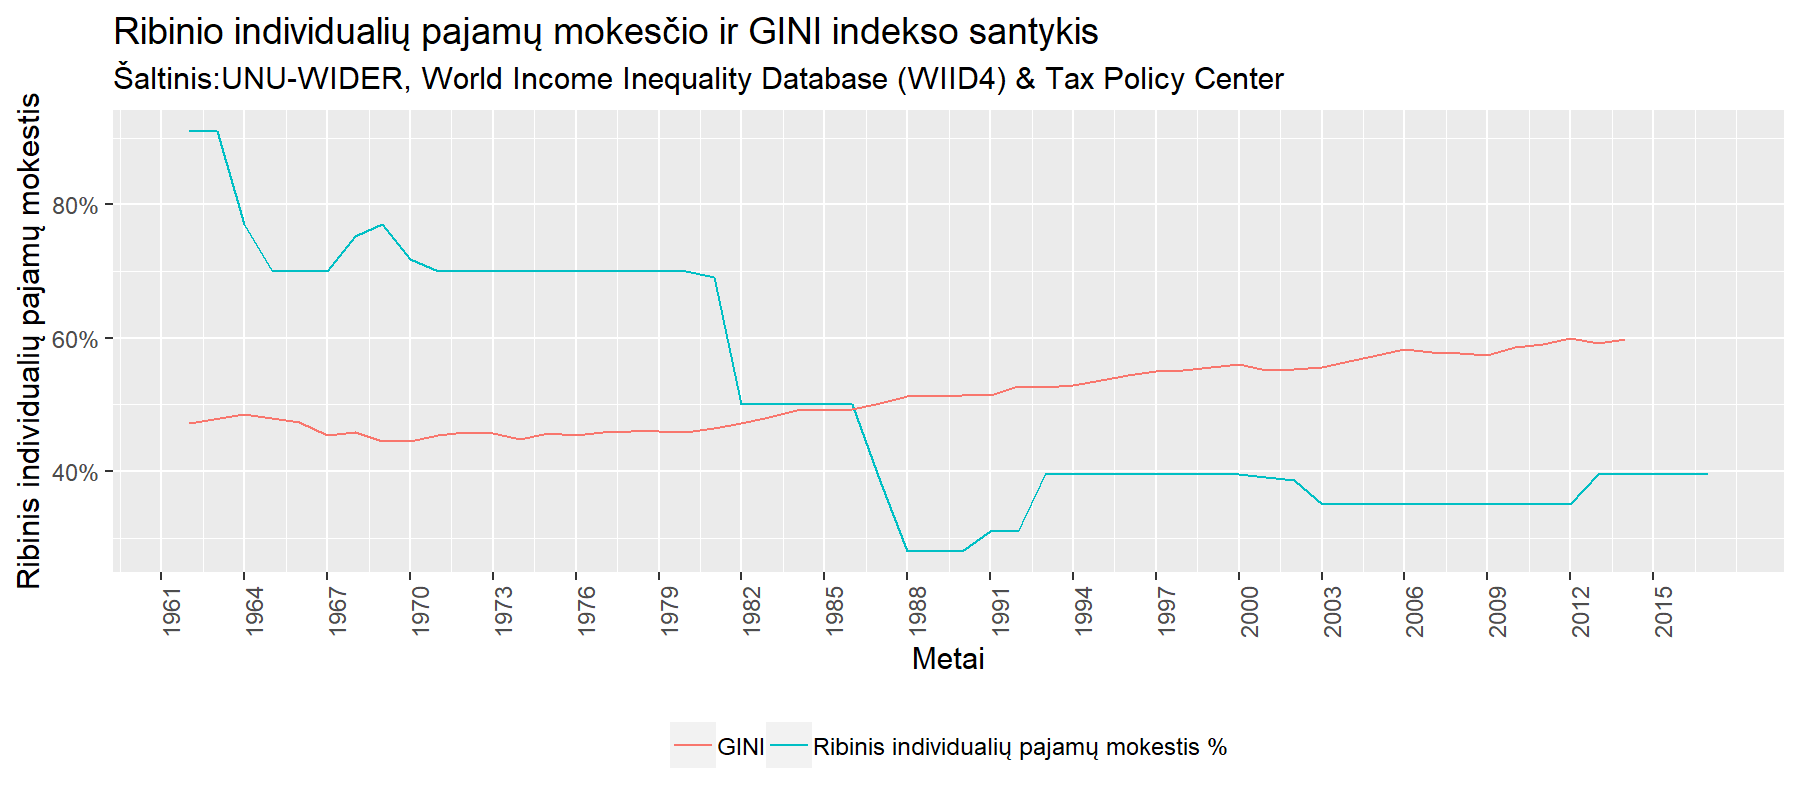
\includegraphics[scale=0.7]{ginivsmarginaltax.png}
\caption{Ribinio individualių pajamų mokesčio ir GINI indekso santykis}
\end{figure}

\subsubsection{Išsilavinimas ir technologijos}
Technologijų tobulėjimas yra įvardijamas kaip viena pagrindinių augančios ekonomikos priežasčių (\cite{jaumotte2013rising}). Nors technologinės inovacijos dažniausiai atsiranda pažangesnėse valstybėse, globalizmo ir laisvos informacijos sklaidos dėka to naudą gali pajausti ir ne tokios išsivysčiusios šalys. Mažėjantys prekybos barjerai per paskutinius 20metų drastiškai paspartino technologinę plėtrą besivystančiose valstybėse. Aukštųjų technologijų importo ir BVP reitingas nuo 1994m padvigubėjo. (\cite{pena2008global}). Nepaisant to, kad technologijos ir globalizacija buvo pasaulinės ekonomikos augimo pastaraisiais dviem dešimtmečiais pamatas, šių veiksnių įtaką pajamų paskirstymo efektyvumui vis dar nėra tiksliai aiški (\cite{jaumotte2013rising}). Technologinis augimas ir Kinijos bei post-sovietinių valstybių integracija į pasaulinės ekonomikos tinklą prisidėjo prie spartaus augimo, tačiau tolygus prieaugio pasiskirstymas nebuvo įgyvendintas. Darbo rinkoje vyksta procesas, kurio metu centrinė didelės vertės ekonominių sektorių ašis pradeda suktis apie aukštesnių ir aukštų įgūdžių bei išsilavinimo reikalaujančius darbus, jų paklausa auga, tuo pačiu automatizacijos procesas mažina nekvalifikuotų, menkų arba vidutinių įgūdžių ir neišsilavinusių darbuotojų poreikį.
Pateiktame grafike (žr.pav.4) analizuojamas dirbančiųjų žmonių lygis pagal išsilavinimą. Nagrinėjamos 3 kategorijos(iki ir pagrindinis išsilavinimas, vidurinis ir aukštesnysis bei aukštasis išsilavinimas) dirbančiųjų Europos Sąjungos šalyse. Matomos stipriai pasireiškiančią aukštąjį išsilavinimą turinčių žmonių užimamos darbo rinkos didėjimo tendeciją bei pagrindinį išsilavinimą turinčių žmonių poreikio darbo rinkoje mažėjimas, kas patvirtina teiginius, jog technologinio tobulėjimo procesas didina pajamų atskirtį tarp skirtingai išsilavinusių žmonių.
\begin{figure}[H]
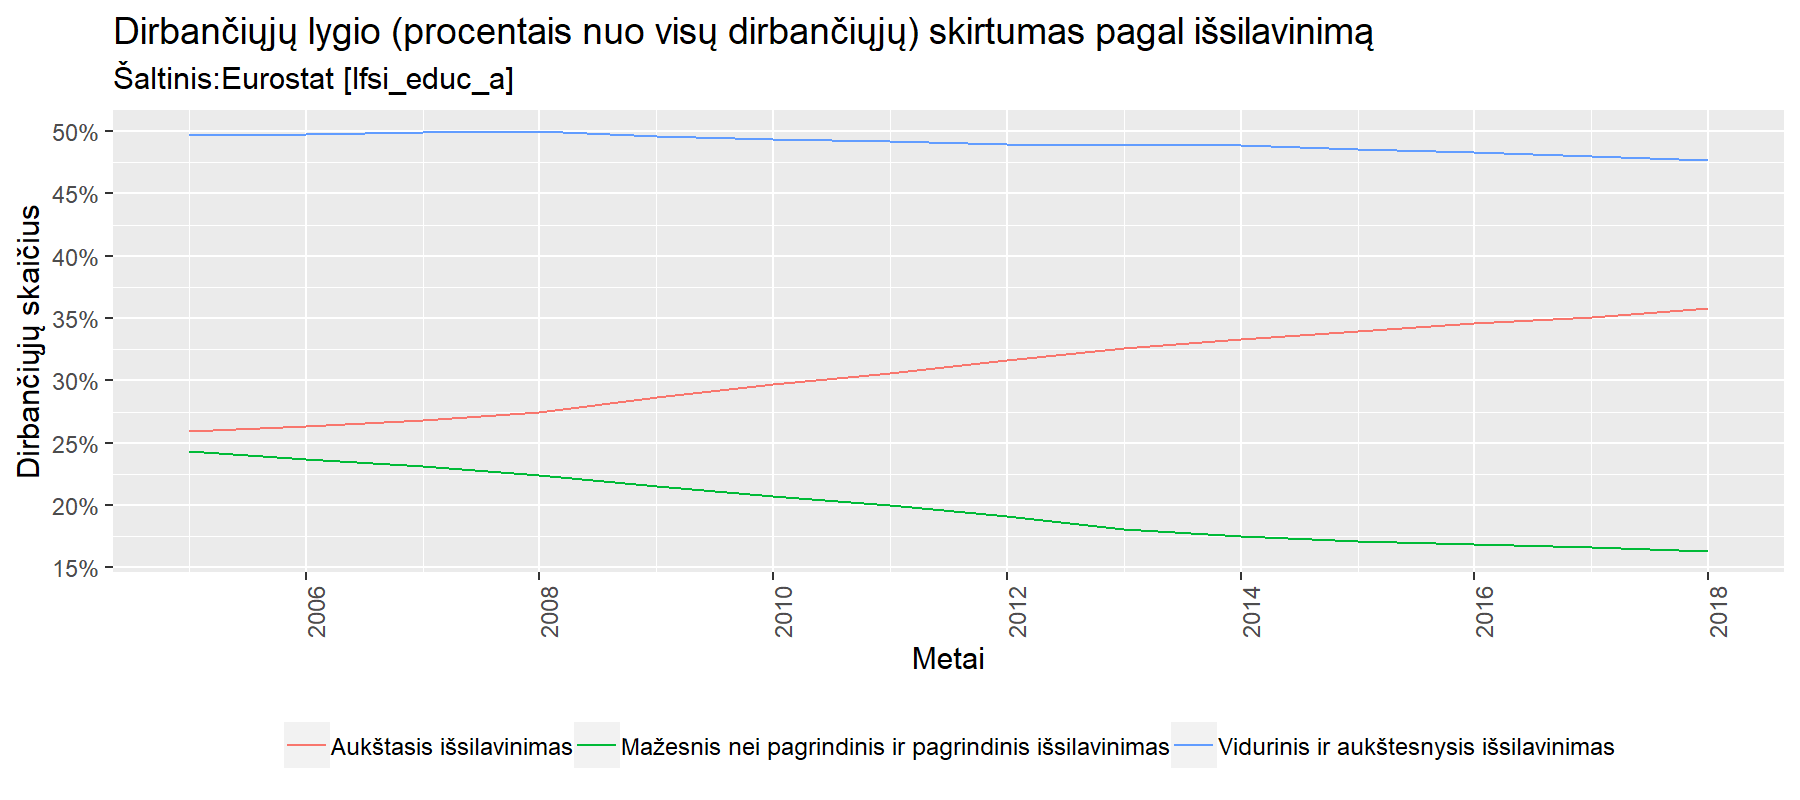
\includegraphics[scale=0.7]{workerseducation.png}
\caption{Dirbančiųjų lygio (procentais nuo visų dirbančiųjų) skirtumas pagal išsilavinimą}
\end{figure}

\subsubsection{Socialiniai Veiksniai}
Pasaulio visuomenė senėja, augant vidutinei gyvenimo trukmei - vis didesnę visuomenės dalį užims vyresnio amžiaus žmonės (žr.pav.5).
\begin{figure}[H]
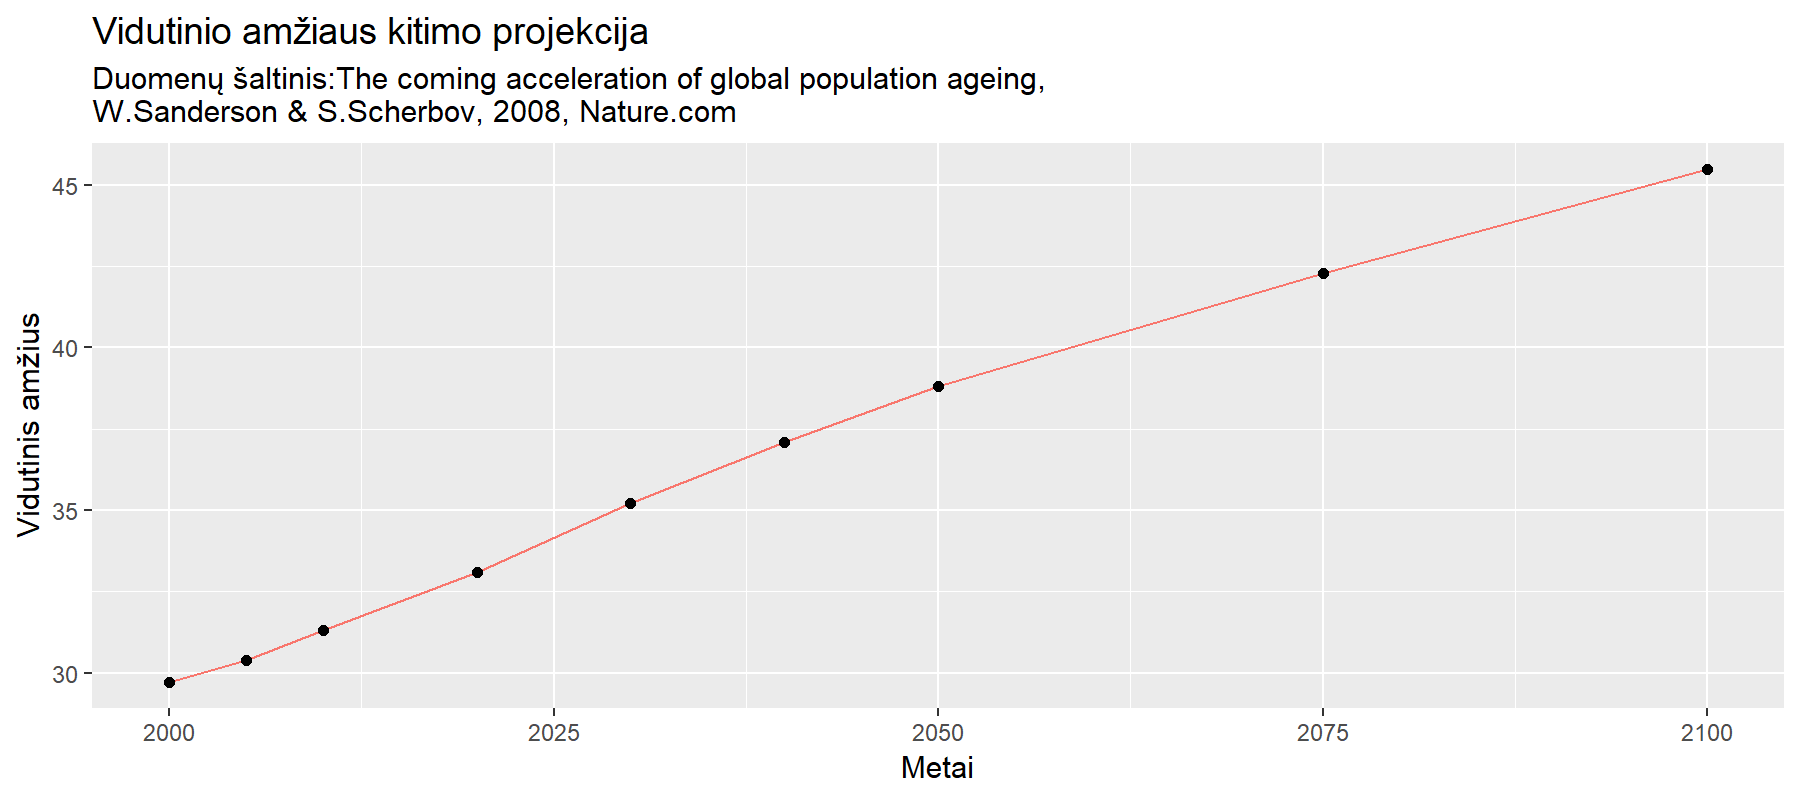
\includegraphics[scale=0.7]{amziausprojekcija.png}
\caption{Vidutinio amžiaus kitimo projekcija}
\end{figure}
Tačiau jie vis dar susiduria su sunkumais integruojantis į darbo rinką. Senyvų žmonių diskriminacija darbo rinkoje mažina jų galimybes didinti savo pajamas. Panaši diskriminacija egzistuoja ir lyčių, kuomet vyrai uždirba daugiau nei moterys, ir neįgaliųjų tarpe, kai negalios diskriminacija trukdo integruotis į darbo rinką. Grafike (žr.pav.6) vaizduojamas vyrų ir moterų uždarbio skirtumo kitimo dinamiką Europos Sąjungos šalyse. Duomenys įrodo faktą, jog atskirties dydis yra reikšmingas, o mažėjimo tempas nėra spartus.
\begin{figure}[H]
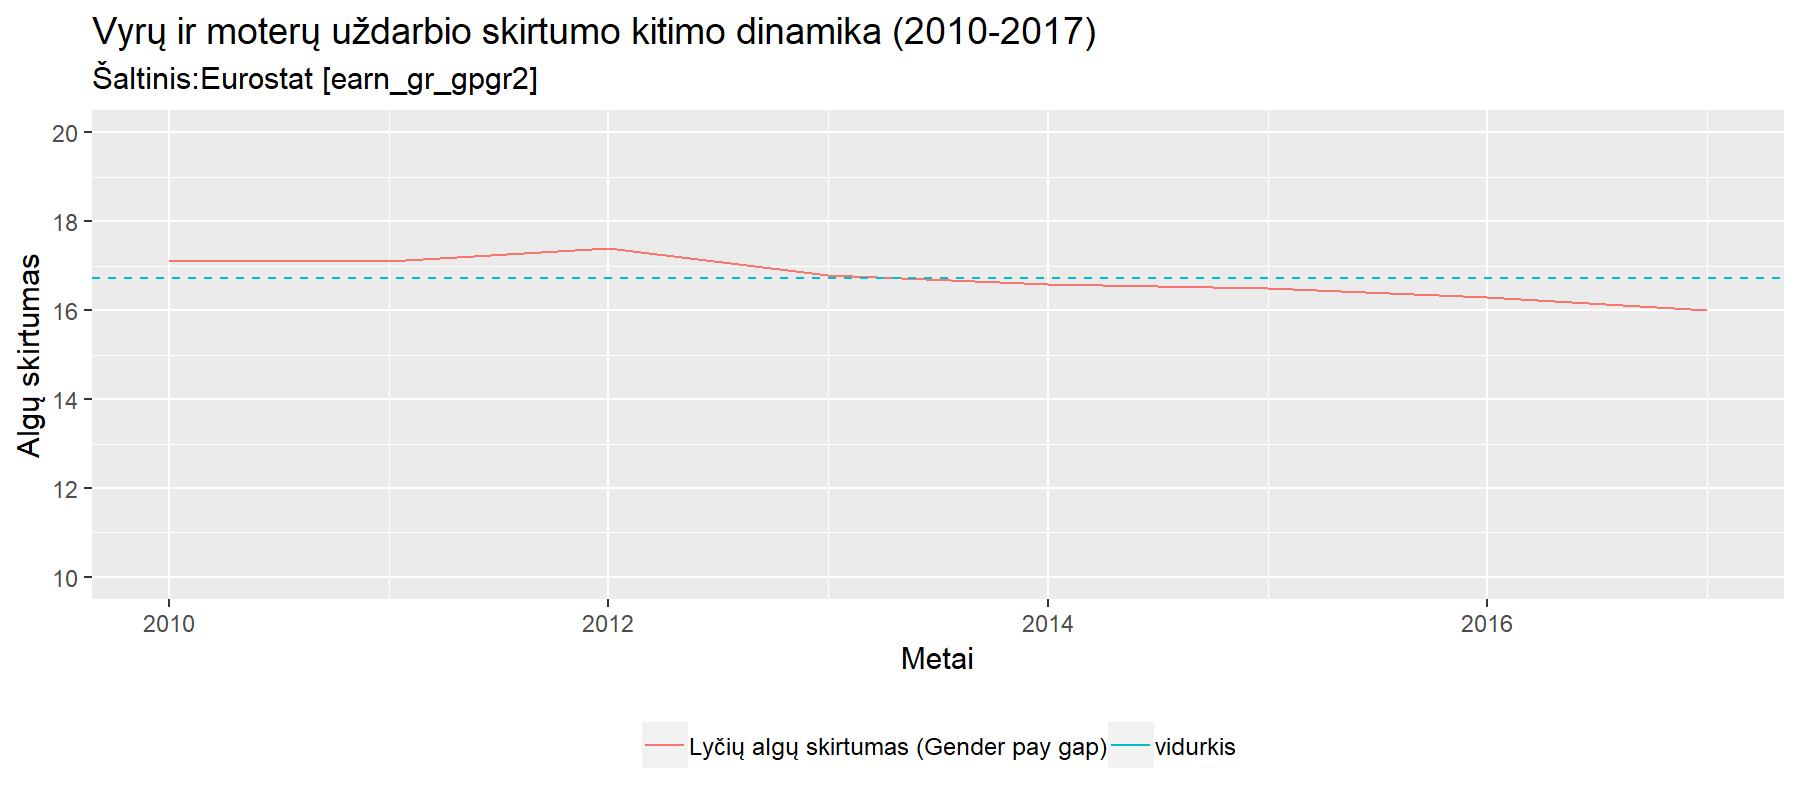
\includegraphics[scale=0.7]{genderpaygap.png}
\caption{Vyrų ir moterų uždarbio skirtumo kitimo dinamika (2010-2017)}
\end{figure}

\section{Pajamų nelygybės mažinimo metodai}
\subsubsection{MMA Didinimas}
MMA - Minimalus mėnesinis atlyginimas. Minimalus atlyginimas vienas iš būdų kovoti su pajamų nelygybe, kadangi minimalaus atlyginimo nustatymas leidžia žmonėms, esantiems pajamų spektro apačioje, pajausti ekonomikos augimą (\cite{litwin2015determining}). Pagrindinė - paskirstymo teorija - leidžia perskirstyti pinigus iš įvairių ekonomikos sektorių mažiau uždirbantiems darbuotojams, tuo pačiu mažinant pajamų nelygybę. Teorija remiasi trimis pagrindiniais pagrindimo mechanizmais:
\begin{enumerate}
\item Minimalios algos pakėlimas padidina prekių ir paslaugų gamybos kaštus, ko pasekoje kyla ir jų kaina. MMA gaunančių darbuotojų perkamoji galia didėja, o kitų pajamų grupių - mažėja, taip skatinama lygybė.
\item Pakėlus MMA, įmonių pelnas mažėja dėl išaugusių gamybos kaštų, todėl mažėja ir akcininkų pajamos.
\item Nors tobulos konkurencijos modelis ir rodo, jog nustačius minimalų atlygį atsiranda priverstinių bedarbių ir kyla nedarbo lygis, tačiau atlikti tyrimai (\cite{cengiz2019effect}) paneigia šios teorijos veikimą realiomis sąlygomis ir teigia, jog MMA kėlimas neturi/beveik neturi jokios įtakos nedarbo lygio kilimui. 
\end{enumerate}
Remiantis (\cite{litwin2015determining}) atlikto tyrimo paremto EBPO (Ekonominio Bendradarbiavimo ir Plėtros Organizacija) priklausančių šalių rezultatais, MMA pakėlimas gali sumažinti pajamų nelygybę, tačiau tik tada, kai minimalus atlygis nustatomas tinkamai remiantis ne nominalia, o realia verte, o norint stabilaus nelygybės mažinimo efekto privaloma sukurti sistema, kuri susietu MMA kitimo dinamiką su infliacijos dydžiu.
Pateiktame grafike (žr.pav.7) nagrinėjama koreliacija tarp minimalaus valandinio atlyginimo ir GINI indekso. Pagal duomenis, galime daryti išvadą, jog sąryšis tarp MMA ir pajamų nelygybės egzistuoja. 
\begin{figure}[H]
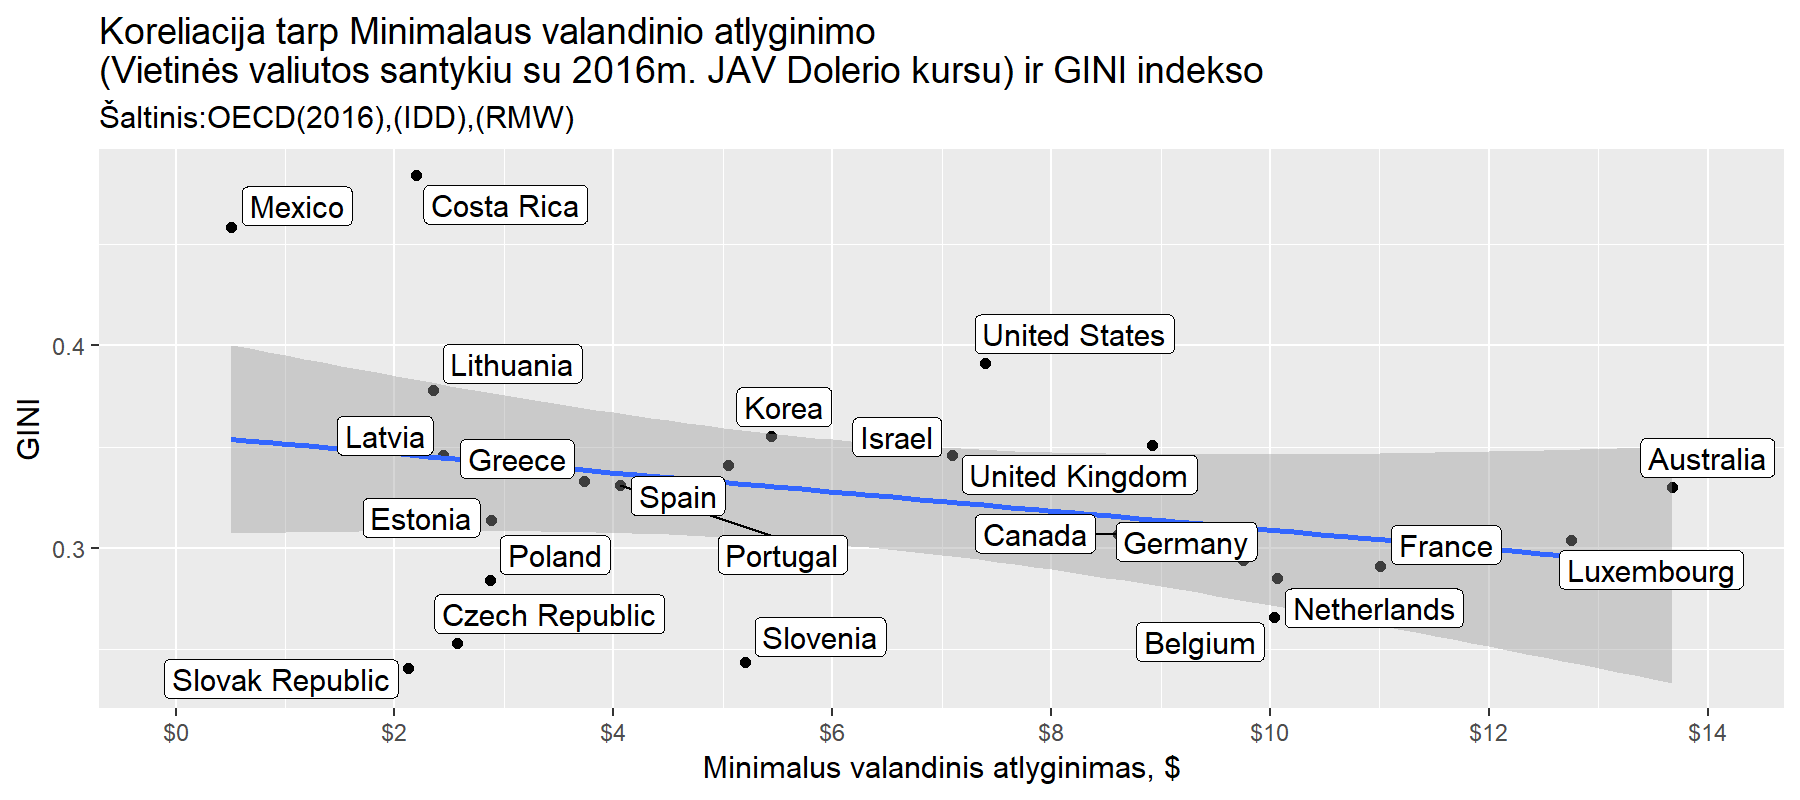
\includegraphics[scale=0.7]{koreliacija.png}
\caption{Koreliacija tarp Minimalaus valandinio atlyginimo (Vietinės valiutos santykiu su 2016m. JAV Dolerio kursu) ir GINI indekso}
\end{figure}

\subsubsection{Mokestinės priemonės ir perskirstymas}
Nors vidutinės trukmės ir ilguoju laikotarpiais naudinga taikyti įgūdžių stokos problemai spręsti skirtas politikos priemones, greitesnio poveikio būtų galima tikėtis pakoregavus mokesčių ir išmokų sistemą. Mokestinė politika gali užimti svarbią rolę paverčiant pajamų po mokesčių paskirstymą lygesniu, taip pat didinant finansavimą kitoms besivystančioms ekonomikos sritimas ar sveikatos ir švietimo sektoriams, kurie reikšmingai gerina žemesnes pajamas gaunančių gyventojų gyvenimo kokybę. 
Pateikti grafikai (žr.pav.8,9) rodo, jog vienus iš didžiausių skirtumą tarp GINI indekso prieš ir po pajamų apmokestinimo turi skandinavijos valstybės, propaguojančios gerovės valstybės modelį, taip pat Austrija, Slovėnija, Belgija, šalys, taikančios progresyvias mokesčių sistemas su aukštu pajamų mokesčio procentu, kas įrodo, jog teisinga mokestinė politika gali reikšmingai mažinti pajamų nelygybės problemą. 
\begin{figure}[H]
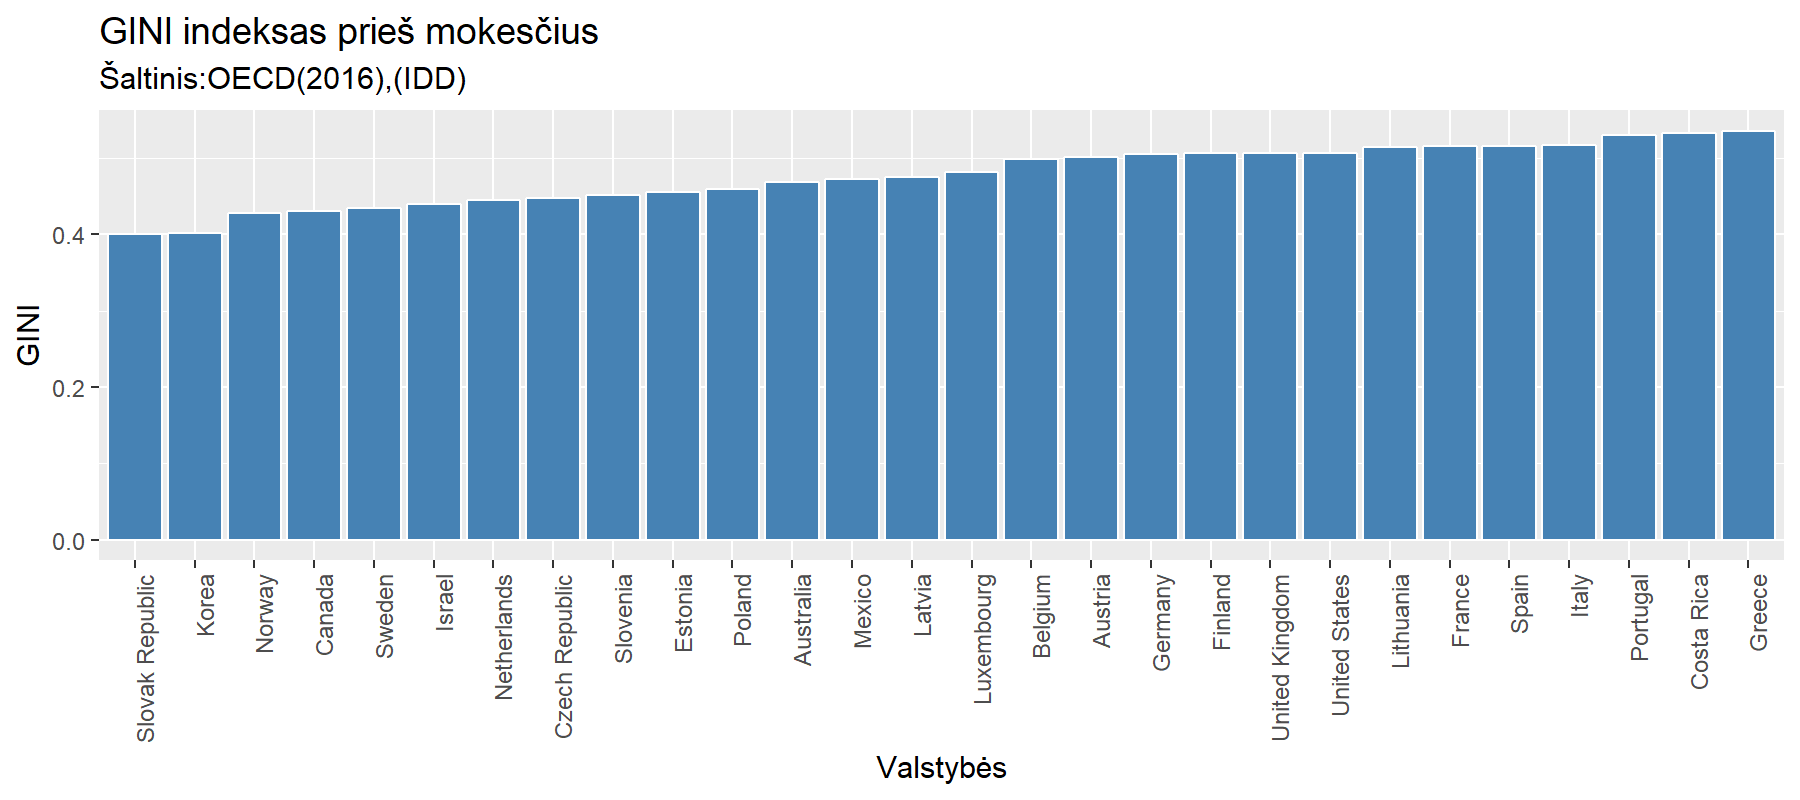
\includegraphics[scale=0.7]{ginibeforetaxation.png}
\caption{GINI indeksas prieš mokesčius}
\end{figure}
\begin{figure}[H]
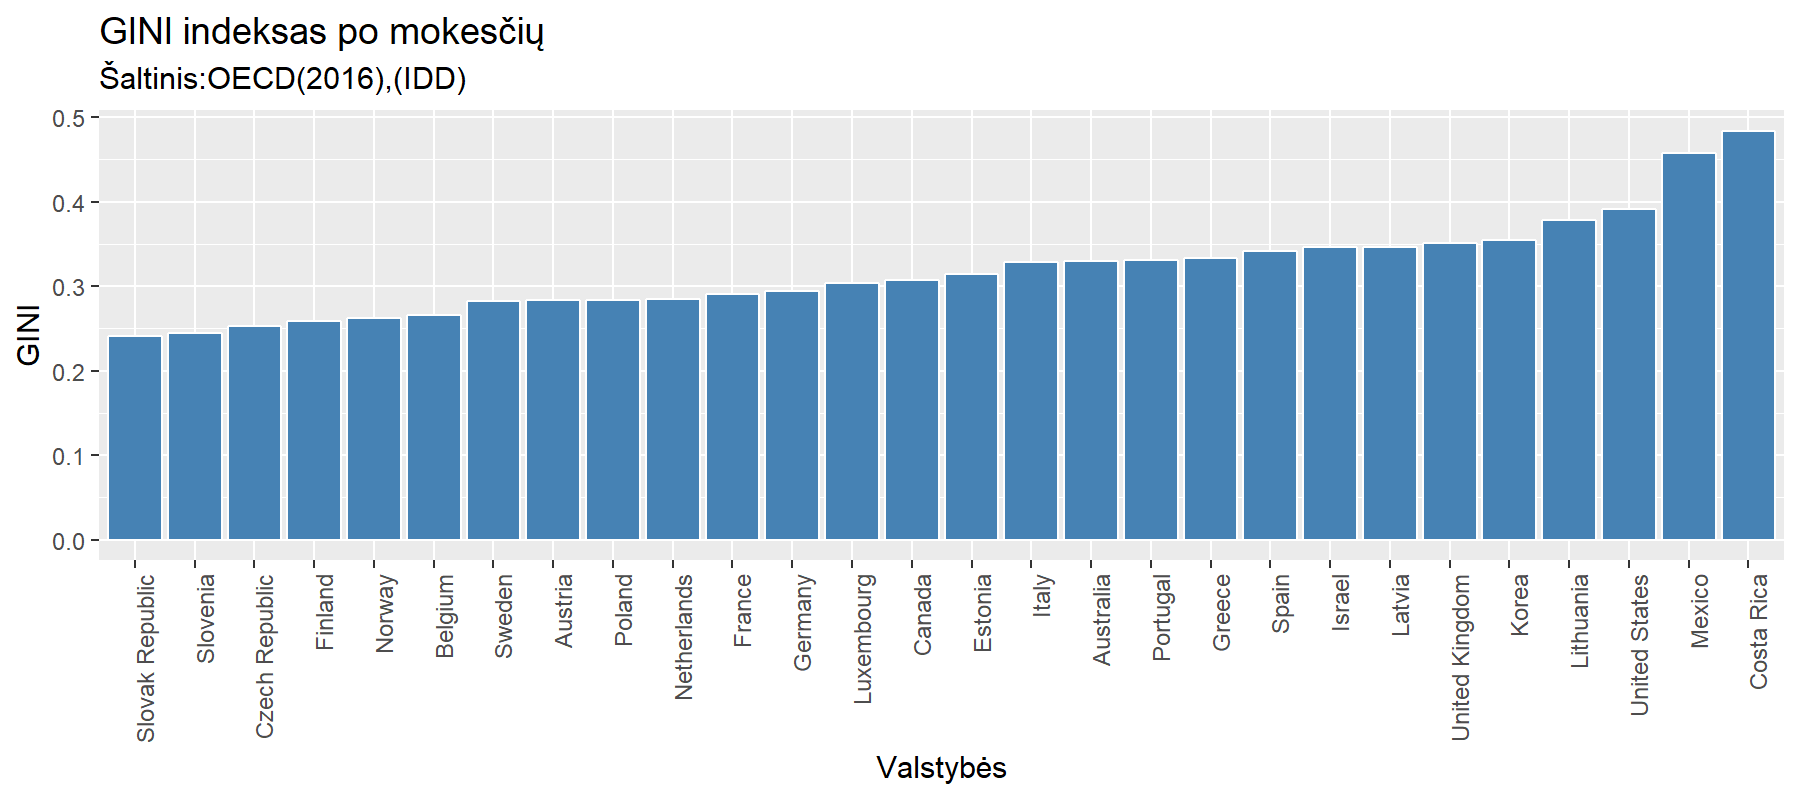
\includegraphics[scale=0.7]{giniaftertaxation.png}
\caption{GINI indeksas po mokesčių}
\end{figure}

\subsubsection{Švietimas ir kompetencijų kėlimas}
Vienas geriausių būdų mažinti nelygybę - invesiticjos į išsilavinimo ir kompetencijų kėlimo galimybes ir jų suteikimas mažesnes pajamas gaunantiems ar žemesnių įgūdžių darbuotojams. Norint naikinti technologijų tobulėjimo ir automatizacijos proceso nulemtus darbo rinkos ir darbo pobūdžio skirtumus, veiksmingiausias būdas - kelti darbuotojų kompetencijas ir atsižvelgiant į tai, kurti naujas darbo vietas. Švietimas veiksmingai padeda kurti lygesnes galimybes vaikams ir jaunimui, jeigu tik visi vaikai, neatsižvelgiant i jų socialinę kilmę, turi galimybę įgyti aukštos kokybės išsilavinimą.
Grafikuose (žr.pav.9,10) nagrinėjama darbuotojų dalyvavusių kompetencijos kėlimo mokymuose ir darbuotojų, kurie domėjosi apie galimybes kelti kvalifikaciją, procentai. Pagal pateiktus duomenis galima daryti išvadą, kad visuomenė vis dar nėra atvira kompetencijų kėlimo kursams (didžiausia dalyvusiųjų reikšmė (<50proc), o nedidelis susidomėjusių šiais kursais procentas leidžia manyti, kad nėra viešos kalbos apie kursų naudą, arba pati kompetencijų kėlimo programa nėra patraukli ir neatrodo teikianti daug naudos. Todėl šioje srityje galimybių sudaryti sąlygas pajamų nelygybės mažinimui tikrai daug.
\begin{figure}[H]
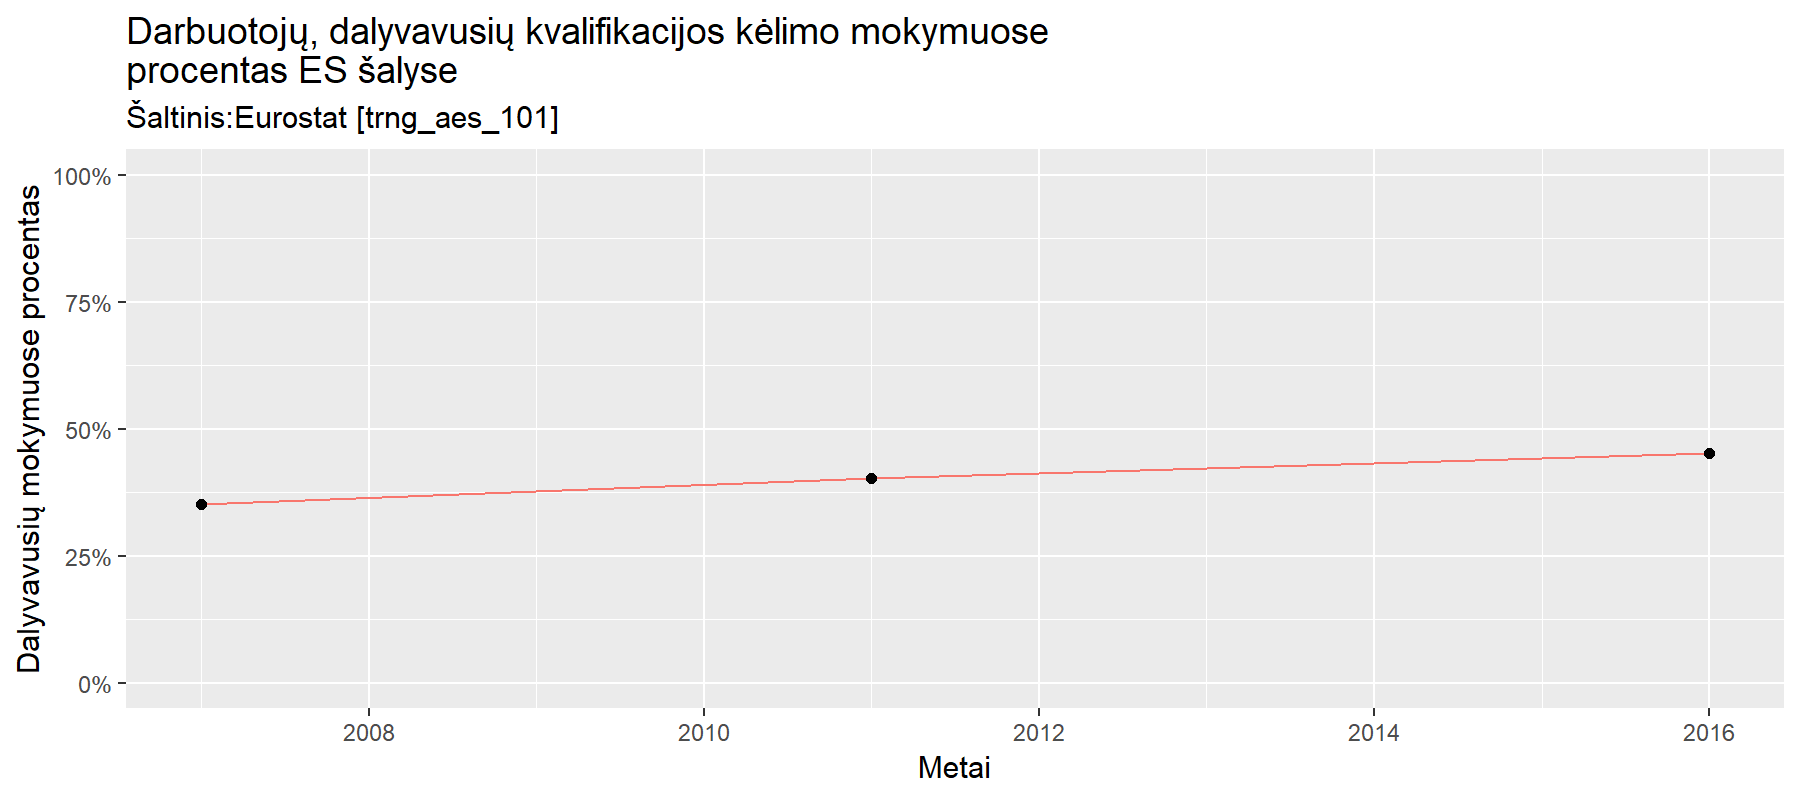
\includegraphics[scale=0.7]{participated.png}
\caption{Darbuotojų, dalyvavusių kvalifikacijos kėlimo mokymuose procentas ES šalyse}
\end{figure}

\begin{figure}[H]
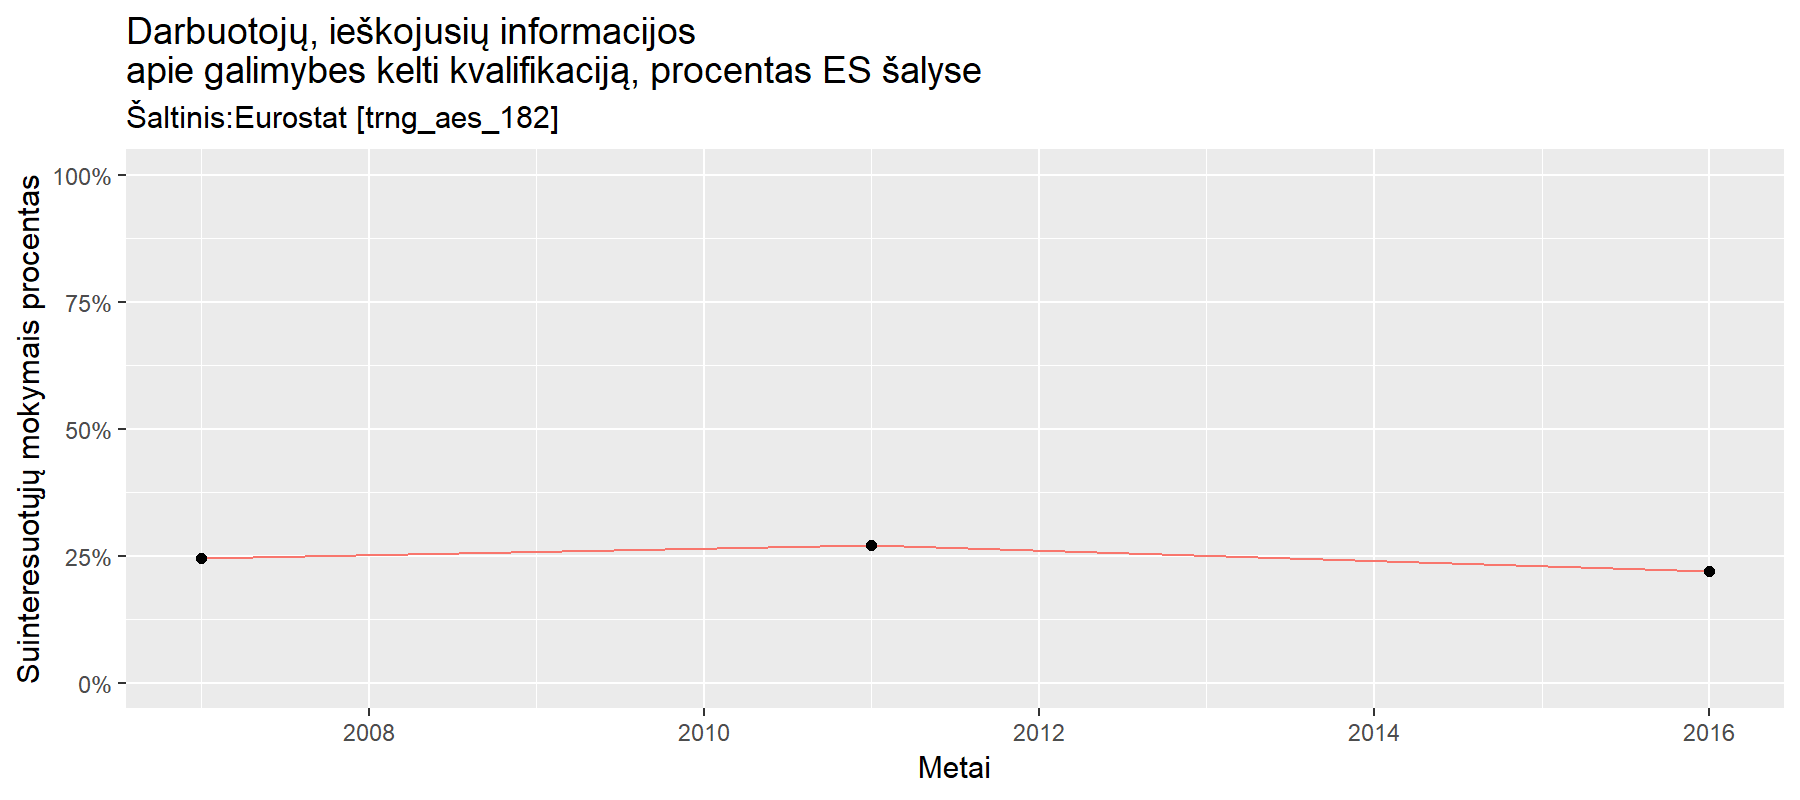
\includegraphics[scale=0.7]{interested.png}
\caption{Darbuotojų, ieškojusių informacijos apie galimybes kelti kvalifikaciją, procentas ES šalyse}
\end{figure}

\newpage

\section{Išvados}
Pajamų nelygybės problemai įtaką daro daug skirtingų faktorių. Nelygybės formavimasis nebuvo trumpojo laikotarpio atsitiktinumas, šį procesą iššaukė tokie faktoriai, kaip: ekonominė santvarka, globalizmas, mokestinės politikos spragos, kompetencijų trūkumas, sparti technologinė raida ar kiti socialiniai veiksniai. Problemos  mąstas per didelis, kad ją būtų galima išspręsti paprastai ir greitai, tačiau ilgalaikių sprendimo būdų yra. Vieni iš jų:   minimalaus mėnesinio atlyginimo progresyvus kėlimas, mokestinių priemonių ir didesnio perskirstymo taikymas bei investicijos į švietimą ir kompetencijų kėlimą. Nors problema vis dar opi, tačiau vieša diskusija ir problemos eskalacija bei struktūrinių pokyčių priėmimas leidžia teikti prielaidą, jog bent EBPO priklausančiose šalyse ateityje atskirtis turėtų mažėti, kiek kitokia situacija mažiau išsyvisčiusiose valstybėse, kur esminių pokyčių gali tekti laukti dar ilgą laiką. 

\newpage
\nocite{*}
\addcontentsline{toc}{section}{Literatūra}
\printbibliography[title={Literatūra}]
\end{document}